%----------createEnumeration----------------------------------------
\op
{createEnumeration}
{creates a new enumeration}
{createEnumeration(Package selectedEObject, String nameValue, String idValue)}
{The package providing the container for the newly created enumeration.}
{
\begin{itemize}
 \item nameValue/newName: The name of the newly created enumeration
 \item idValue/newID: The id of the newly created enumeration
\end{itemize}
}
{There is no enumeration whose name equals the parameter-value of 'newName' (see
\ref{subsec:checkOtherNames})}
{Only the name and the id will be set via input data. Visibility will be set
with a default value as defined with the diagram editor in the image below.}
\begin{figure}[H]
  \centering
  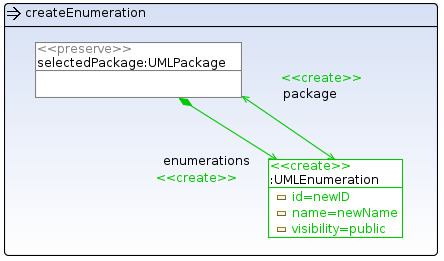
\includegraphics[width=0.65\textwidth]{pics/createEnumeration.png}
  \caption{createEnumeration}
  \label{createEnumeration}
\end{figure}
%----------deleteEnumeration----------------------------------------
\op
{deleteEnumeration}
{Deletes an enumeration}
{deleteEnumeration(Enumeration selectedEObject)}
{The enumeration which should be deleted}
{-}
{-}
{For a better readability this is a simplified version of the
'deleteEnumeration'-transformation and will only cover cases where the
enumeration has no containments and no references to other elements. Such a
complex transformation rule exits but won't be listed here.}
\begin{figure}[H]
  \centering
  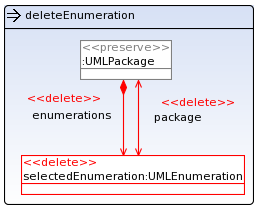
\includegraphics[width=0.4\textwidth]{pics/deleteEnumeration_emptyAndUnreferenced.png}
  \caption{deleteEnumeration}
  \label{deleteEnumeration}
\end{figure}
%----------editEnumerationName----------------------------------------
\op
{editEnumerationName}
{edits the name of an enumeration}
{editEnumerationName(Enumeration selectedEObject, String nameValue)}
{The enumeration whose name should be renamed.}
{
\begin{itemize}
 \item nameValue/newName: The new name
\end{itemize}
}
{There is no enumeration in the same package whose name equals the parameter-value of
'newName' (see
\ref{subsec:checkOtherNames})}
{The \textless\textless create\textgreater\textgreater  -symbol in the image
means that even if the attribute exists its value will be overwritten.
'newName' is the placeholder for the input name.}
\begin{figure}[H]
  \centering
  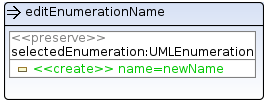
\includegraphics[width=0.4\textwidth]{pics/editEnumerationName.png}
  \caption{editEnumerationName}
  \label{editEnumerationName}
\end{figure}
%----------editEnumerationVisibility----------------------------------------
\op
{editEnumerationVisibility}
{edits the visibility of an enumeration}
{editEnumerationVisibility(Enumeration selectedEObject, Visibility visibilityValue)}
{The enumeration whose visibility should be edited.}
{
\begin{itemize}
 \item visibilityValue/visibility: The new visiblility
\end{itemize}
}
{-}
{The \textless\textless create\textgreater\textgreater  -symbol in the image
means that even if the attribute exists its value will be overwritten.
'visibility' is the placeholder for the input visibility value.}
\begin{figure}[H]
  \centering
  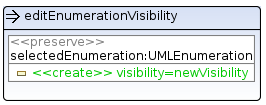
\includegraphics[width=0.4\textwidth]{pics/editEnumerationVisibility.png}
  \caption{editEnumerationVisibility}
  \label{editEnumerationVisibility}
\end{figure}
%----------moveEnumeration----------------------------------------
\op
{moveEnumeration}
{moves an enumeration from a package to another package}
{moveEnumeration(Enumeration selectedEObject, Package tgt)}
{The enumeration which should be moved.}
{
\begin{itemize}
 \item tgt/tgt[moveEnumeration]: the target package
\end{itemize}
}
{There is no enumeration with the same name in the target context (see
\ref{subsec:checkOtherNames})}
{Only references will change.}
\begin{figure}[H]
  \centering
  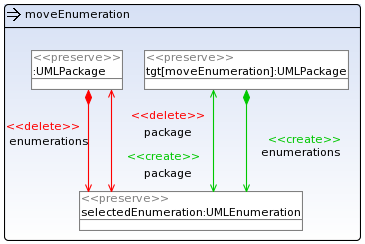
\includegraphics[width=0.65\textwidth]{pics/moveEnumeration.png}
  \caption{moveEnumeration}
  \label{moveEnumeration}
\end{figure}